\documentclass[../main.tex]{subfiles}
\graphicspath{{\subfix{../src/}}}

\begin{document}

Due to the training dataset \cite{kinmusdataset} from section \ref{sec:dataset},  containing joint angles as ground truth, both methods are trained as regression networks rather than classification networks, and are trained using Mean Square Error (MSE) loss.

The main objective of these tests...

\subsubsection{Machine-Learning Designs}

%TODO: Some introduction and explanation of feature extraction, what types and papers that uses these.
%TODO: Some introduction and explanation of SVM and LDA types of networks.
%TODO: Go back and see what papers uses these.

%\subsection{Software Hand Design}

\section{Tests \& Results}

Due to the problems with the Motive motion capture software explained in section \ref{sec:motiveproblems}, it was determined that the main dataset for training the chosen methods would be based on dataset \cite{kinmusdataset} from the paper \cite{jarque2019}.
The dataset created during the development of this thesis will be used as an additional test. 
The dataset has been pre-processed using a 4th-order bandpass filter with a band of  $25$ to $500Hz$, then the data was subject to a 4th-order low-pass filter at $8 Hz$.


\subsection{Feature-Based Multi Layer Perceptron Network}

Neural Networks are widely used in the field of AI.
One type of widely used neural network is a fully-connected Multi-Layer Perceptron (MLP) Network.
The MLP network is popular due to its structure and training capabilities.
A MLP consists of layers of weighted activation functions where each activation function in a layer recieves the entire previous layer's output summed up as input.
Due to the structure of a MLP, the network is capable of recieving a set of inputs and be trained to approximate a n'th degree polynomial function that relates the given inputs and outputs.
The network is trained by updating the individual weights through backpropagation with the predicted output and a ground-truth output.
The MLP network could be used to predict the relation between muscle activity and finger movements.

%In order to initially test the the dataset, a simple MLP network will be trained as a baseline for performance, and for testing the general applicability of window-based networks.



\subsection{Windowed Convolusional Neural Networks}

An alternative to a MLP that is similar in functionality is a Convoluted Neural Network (CNN).
A CNN consists of a set of Convolutional Layers that deforms inputs to abstract convolution features.
The structure is considered sparcely connected due to the convolution layers are only recieving a subset of the previous convolution features.
The feature conversion is ideal when a network needs to become robust and needs to recognize larger concepts in the input.
This functionality is especially used when the input data takes the shape of a matrix.
Once the input is convoluted to a chosen feature abstraction, it is given to a MLP strucure trained to convert the convolution features into a useable output.
%TODO: needs sources for this stuff?
%TODO: Go back and see what papers uses CNN's
CNN networks have no buildin time-based functionality, they recieve a set of inputs and produce an output.
It is possible however to represent time if the input is given in segments consisting of multiple timeframes.
Because of this, the sEMG muscle activity from the dataset is segmented into windows of a desired size, the output angles that the network should do regression towards are then chosen to be the first angle after the window.
%TODO: Images of these for better clarity!!!!
A CNN network can be used in the field of sEMG processing due to the convolution layer's ability to learn abstract formations of the sEMG data.
The network would be able to identify patterns in sEMG data and correlate them to an appropoate output.
%TODO: formations? another word?
For this test, a CNN network is created that has the network structure seen in figure \ref{fig:cnn_structure}.

\begin{figure}[h]
\begin{center}
\includegraphics[width=0.8\textwidth]{example-image-a}
\caption{Chosen CNN network structure.}
\label{fig:cnn_structure}
\end{center}
\end{figure}
%TODO: figure of network

As visualized in the figure, the CNN network consists of 3 Convolution layers followed by two MLP layers.
The Convolution layers extract features up to a size of 
%A CNN is trained on the network, using a window size of 40 samples were used.
%TODO: Give example of a state-of-the-art paper CNN as an alternative to mine!!!



%TODO: this is not a good way to show results!
%\begin{figure}[h]
%\begin{center}
%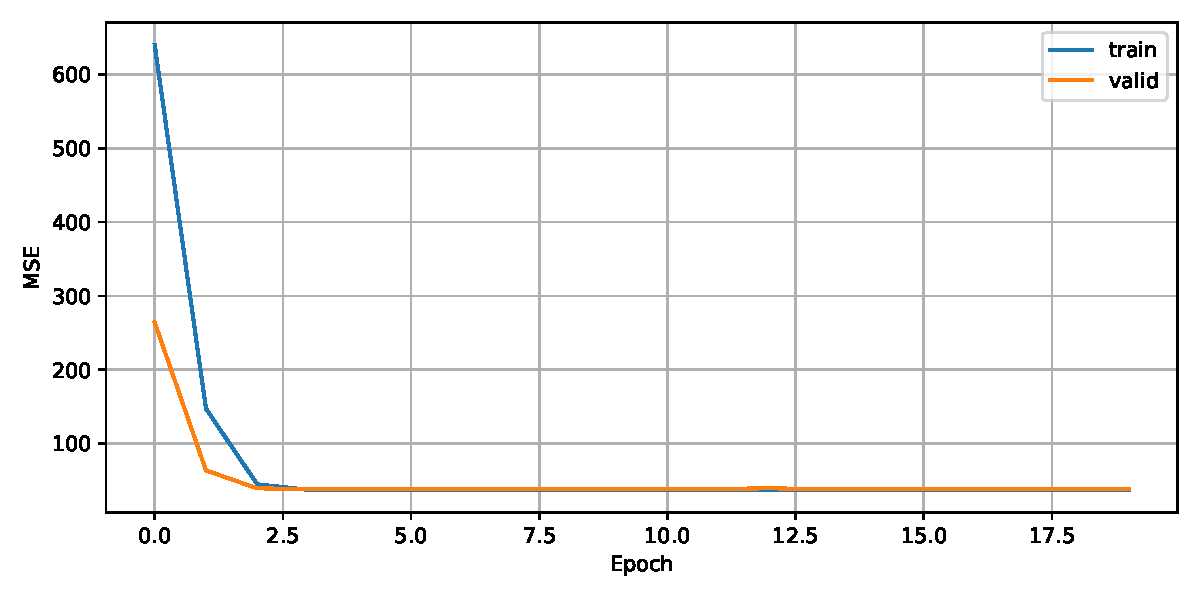
\includegraphics[width=0.99\textwidth]{cnn_trainvalid.pdf}
%\caption{Example figure text}
%\label{fig:cnntrainvalid}
%\end{center}
%\end{figure}
%
%\begin{figure}
%    \centering
%    \begin{subfigure}[b]{0.49\textwidth}
%        \centering
%        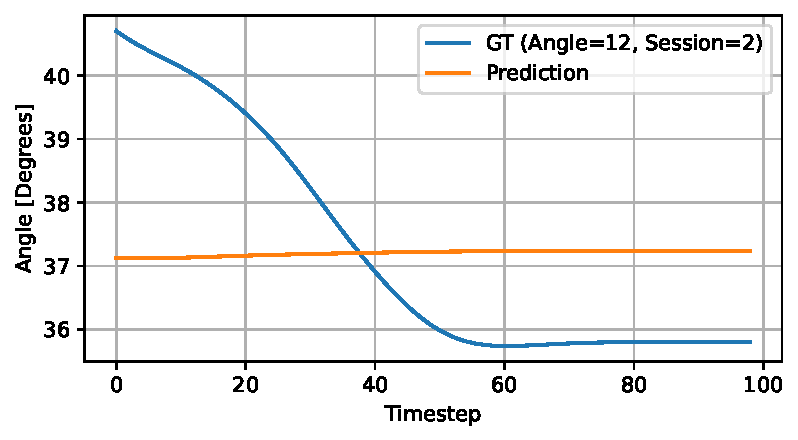
\includegraphics[width=\textwidth]{CNNtest0.pdf}
%        \caption{}
%        \label{fig:y equals x}
%    \end{subfigure}
%    \hfill
%    \centering
%    \begin{subfigure}[b]{0.49\textwidth}
%        \centering
%        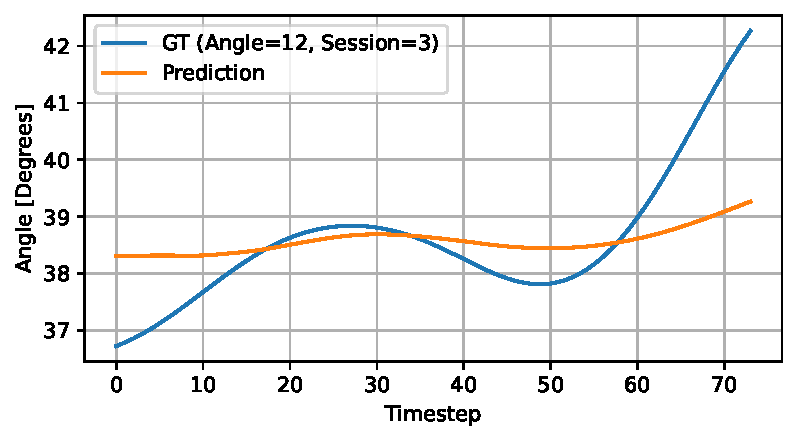
\includegraphics[width=\textwidth]{CNNtest1.pdf}
%        \caption{}
%        \label{fig:y equals x}
%    \end{subfigure}
%    \hfill
%    \begin{subfigure}[b]{0.49\textwidth}
%        \centering
%        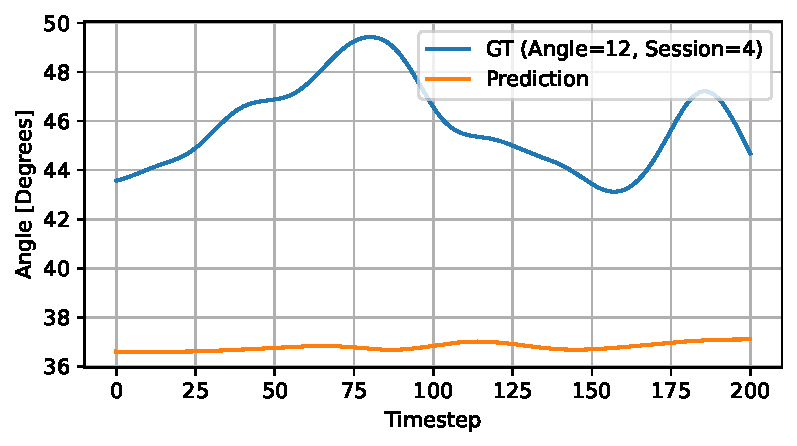
\includegraphics[width=\textwidth]{CNNtest2.pdf}
%        \caption{}
%        \label{fig:three sin x}
%    \end{subfigure}
%    \hfill
%    \begin{subfigure}[b]{0.49\textwidth}
%        \centering
%        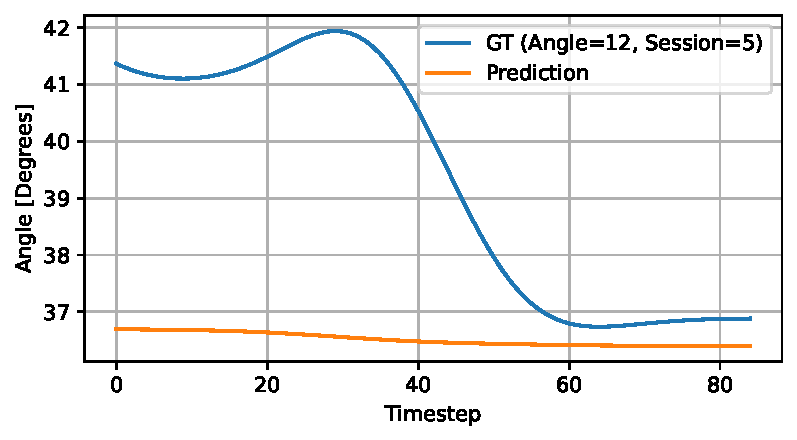
\includegraphics[width=\textwidth]{CNNtest3.pdf}
%        \caption{}
%        \label{fig:five over x}
%    \end{subfigure}
%    \hfill
%    \begin{subfigure}[b]{0.49\textwidth}
%        \centering
%        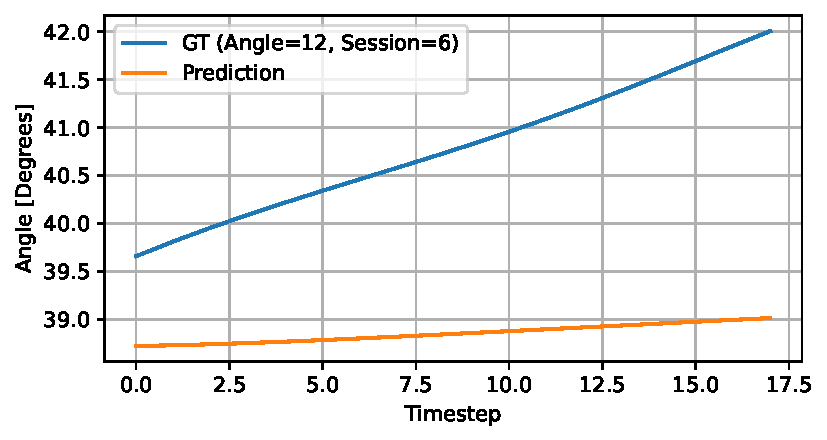
\includegraphics[width=\textwidth]{CNNtest4.pdf}
%        \caption{}
%        \label{fig:five over x}
%    \end{subfigure}
%    \hfill
%    \begin{subfigure}[b]{0.49\textwidth}
%        \centering
%        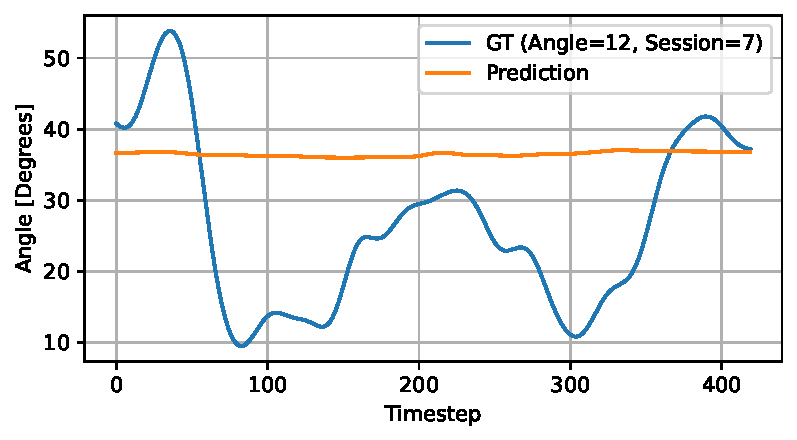
\includegraphics[width=\textwidth]{CNNtest5.pdf}
%        \caption{}
%        \label{fig:five over x}
%    \end{subfigure}
%    \hfill
%    \caption{Regression of Finger angles using a CNN network.}
%    \label{fig:CNNregression}
%\end{figure}



%\subsubsection{Pre-Processing Filters}
%\textbf{Method}\\
%\textbf{Test}\\
%\textbf{Results}\\
%
%\subsubsection{Window Size}
%\textbf{Method}\\
%\textbf{Test}\\
%\textbf{Results}\\
%
%\subsubsection{Training Parameters}
%\textbf{Method}\\
%\textbf{Test}\\
%\textbf{Results}\\
%
%\subsubsection{Types of Features for extraction}
%\textbf{Method}\\
%\textbf{Test}\\
%\textbf{Results}\\
%
%\subsection{3. Recurrent Neural Networks}
%
%\subsubsection{Training Parameters}
%\textbf{Method}\\
%\textbf{Test}\\
%\textbf{Results}\\
%
\subsubsection{Recurrent Neural Networks}

Network types ideal for time-based data are Recurrent Neural Networks (RNN).
RNN networks are similar to MLP's with the main difference being that a RNN keeps a hidden memory state that is derived from earlier inputs.
This functionality makes RNN networks ideal for concurrent, time-based systems where a sequencial input distribution needs to be converted to a output regression.  
Additionally, since the RNN network does not use a window of data, it would be able to have a quicker response time than a MLP or a CNN.

A variant of a RNN can contain a special kind of hidden memory called Long Short Term Memory (LSTM).
a LSTM uses gates as a way of containing a memory.

%TODO: Some introduction and explanation of RNN and LSTM types of networks.
%TODO: Go back and see what papers uses these.

%\subsection{(Machine Learning Algorithms)}
%%TODO: Determine what algorithms i want here
%
%\subsubsection{Types of Features for extraction}
%\textbf{Method}\\
%\textbf{Test}\\
%\textbf{Results}\\



\subsection{Useability of the Simulated Prosthetic Hand}

Existing prosthetic hand simulations are not possible to get access to, as explained in section \ref{sec:hand_alternatives}, they are either unavailable through deprecation or pay-to-acces by buying a real prosthetic.
Due to non-availability of prosthetic hand simulations, it was chosen that through this thesis, a open source prosthetic hand needed to be created for testing of the algorithms developed as part of this project.
The prosthetic hand created for this thesis can be seen in section \ref{sec:prost_sim}.
The prosthetic was designed to be as anatomically similar as a real hand as possible.
This was done in order to accurately simulate the movement of a real hand.
%TODO: Is this intro good?

\subsubsection{Anatomical Assessment and Maneuverability}

The useability and moveability of the simulated prosthetic hand needs to be assessed.

\textbf{Method}\\
As an initial test, it is reasonable to test if the hand is able to acheive the end poses of the grip types from section \ref{sec:dataset} table \ref{tab:grips}. 

\textbf{Test \& Results}\\

The hand was manually posed into all 4 grip types, and visually compared, as can be seen in figure  \ref{fig:hand_pose_test}.

%TODO: Needs to be a figure of figures!
\begin{figure}[h]
\begin{center}
\includegraphics[width=0.8\textwidth]{example-image-a}
\caption{Example figure text}
\label{fig:hand_pose_test}
\end{center}
\end{figure}

Based on a visual comparison of figure \ref{fig:hand_pose_test}, it can be concluded that the prosthetic hand is able to be posed similarly to the real-life refrence.
It can be seen how the prosthetic is porpotionally correct and thus also allows for accurate posing when posed manually.

\subsubsection{Posing based on Network Output}

As a result of testing different network types and their applicability for creating suitable motorcontrol output for a prosthetic hand, it would be ideal to test the network output on the prosthetic simulation.
For full video see appendix ??.
%TODO: Insert appendix here

\textbf{Method}\\

\textbf{Test \& Results}\\



%\subsection{Method 1: Windowed CNN}
%\subsection{Test 1: Windowed CNN}
%\subsection{Results 1: Windowed CNN}
%\subsection{Method 2: RNN}
%\subsection{Test 2: RNN}
%\subsection{Results 2: RNN}


%TODO: see Zhaolong2021 (page 10) for example of how to compare MSE for different neuron amounts, even for multiple subjects!

\end{document}
